\documentclass[pscyr]{hedlab}
\usepackage[russian]{babel}
\usepackage{graphicx}
\graphicspath{{images/}}
\usepackage{listings}

\lstset{
    basicstyle=\footnotesize,
    inputencoding=utf8,
    extendedchars=True,
    language=[Sharp]C,
    numbers=left,
    numberstyle=\footnotesize,
    breakatwhitespace=\false,
    breaklines=True,
    tabsize=2,
    keepspaces=true,
}

\labname{Публикация данных в Web\\Часть 2}
\labnum{4}
\student{Голубев~А.~В., САПР-1.1п}
\labdate{}

\begin{document}
    \makeheader
    \emph{Цель:} получить практические навыки добавления, редактирования и удаления данных из 
    веб-приложения с использованием компонент SQLDataSource и GridView.\\
    \emph{Задачи:} 
    \begin{enumerate}
        \item Создать базу данных из связанных таблиц произвольной предметной области.
        \item Осуществить подключение к базе данных с использованием компонент SQLDataSource.
        \item Отобразить данные с помощью объекта класса GridView.
        \item Реализовать метод добавления данных в таблицу базы данных.
        \item Реализовать метод корректировки данных в таблице базы данных непосредственно в 
            объекте класса GridView.
        \item Реализовать метод удаления данных из таблицы базы данных.
    \end{enumerate}
    Реализация работы с таблицой БД:
    \lstinputlisting{./code/code.cs}
    \pagebreak
    Страница с элементами GridView и SqlDataSource:
    \lstinputlisting[inputencoding=utf8,basicstyle=\footnotesize,language=HTML]{./code/page.aspx}

    \pagebreak
    Скриншоты с Web-страниц с БД:
    \begin{figure}[h!]
        \center
        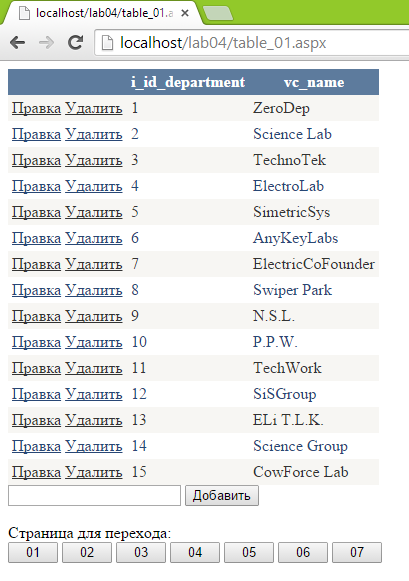
\includegraphics[width=.47\textwidth]{lab04_01} \hspace{1em}
        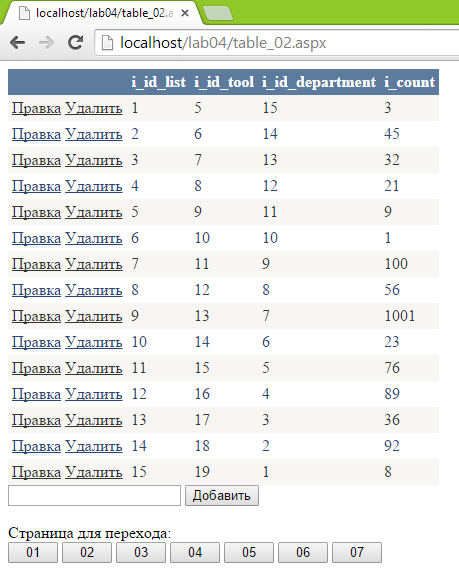
\includegraphics[width=.47\textwidth]{lab04_02} \\
        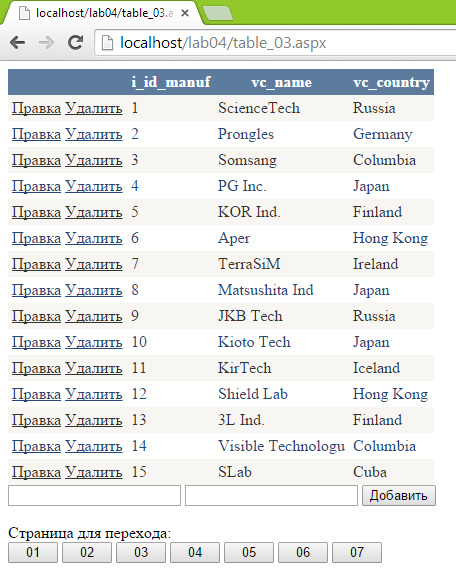
\includegraphics[width=.47\textwidth]{lab04_03} \hspace{1em}
        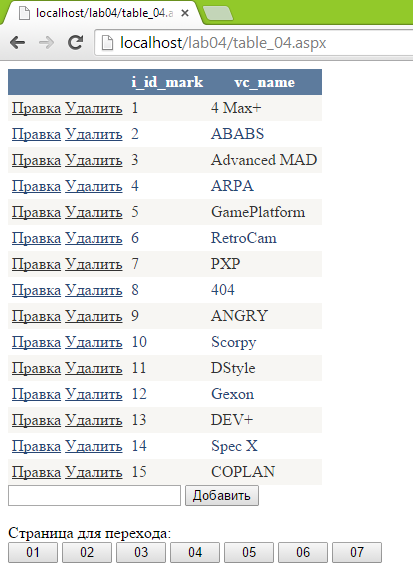
\includegraphics[width=.47\textwidth]{lab04_04}
    \end{figure}
    \pagebreak
    \begin{figure}[h!]
        \center
        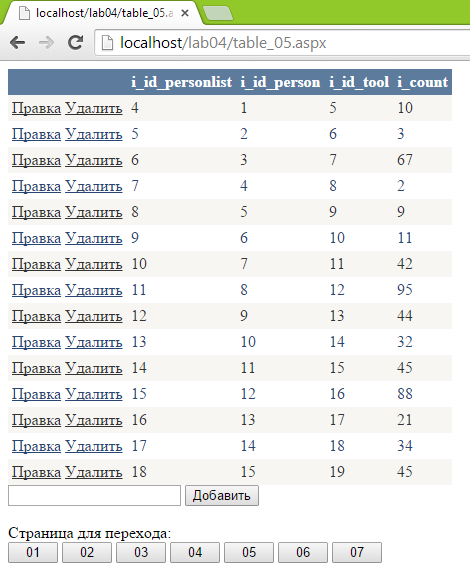
\includegraphics[width=.47\textwidth]{lab04_05} \hspace{1em}
        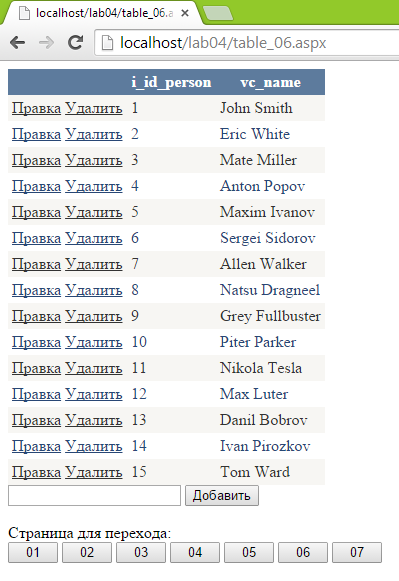
\includegraphics[width=.47\textwidth]{lab04_06} \\
        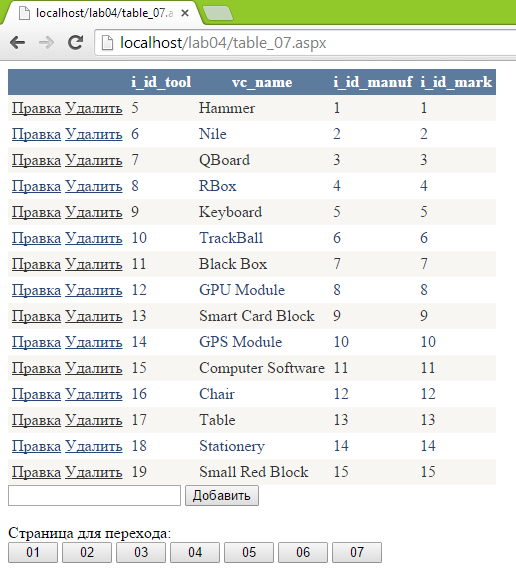
\includegraphics[width=.47\textwidth]{lab04_07}
    \end{figure}
    \pagebreak

    \emph{Вывод:} в результате проделанной работы
    \begin{enumerate}
        \item Создал базу данных из связанных таблиц произвольной предметной области.
        \item Осуществили подключение к базе данных с использованием компонент SQLDataSource.
        \item Отобразили данные с помощью объекта класса GridView.
        \item Реализовали метод добавления данных в таблицу базы данных.
        \item Реализовали метод корректировки данных в таблице базы данных непосредственно в объекте 
        класса GridView.
        \item Реализовали метод удаления данных из таблицы базы данных.
    \end{enumerate}
\end{document}